\begin{figure}[htb!]
  \centering
  \begin{subfigure}{0.14\textwidth}
    \caption*{Mode of agitation}
  \end{subfigure}
  \hspace{0.02\textwidth}
  \begin{subfigure}{0.14\textwidth}
    \caption*{\protect\raggedright Experimental crack network}
  \end{subfigure}
  \hspace{0.02\textwidth}
  \begin{subfigure}{0.15\textwidth}
    \caption*{$\Gc^*$}
    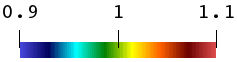
\includegraphics[width=\textwidth]{Chapter4/figures/rainbow_horizontal.png}
  \end{subfigure}
  \begin{subfigure}{0.15\textwidth}
    \caption*{$\psi_c^*$}
    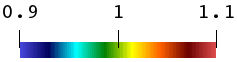
\includegraphics[width=\textwidth]{Chapter4/figures/rainbow_horizontal.png}
  \end{subfigure}
  \begin{subfigure}{0.15\textwidth}
    \caption*{$d$}
    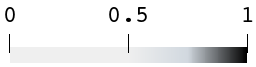
\includegraphics[width=\textwidth]{Chapter4/figures/grayscale_horizontal.png}
  \end{subfigure}
  
  \begin{subfigure}{0.14\textwidth}
    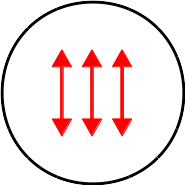
\includegraphics[width=\textwidth]{Chapter4/figures/2D/brick_schematic.png}
    \caption{}
  \end{subfigure}
  \hspace{0.02\textwidth}
  \begin{subfigure}{0.14\textwidth}
    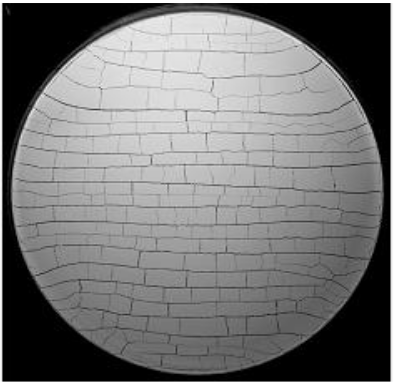
\includegraphics[width=\textwidth]{Chapter4/figures/2D/paste_brick.png}
    \caption{}
  \end{subfigure}
  \hspace{0.02\textwidth}
  \begin{subfigure}{0.15\textwidth}
    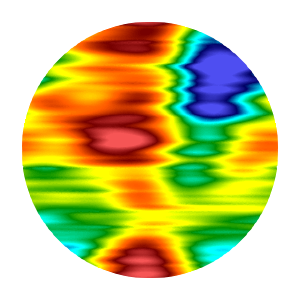
\includegraphics[width=\textwidth]{Chapter4/figures/2D/Gc_brick.png}
    \caption{}
  \end{subfigure}
  \begin{subfigure}{0.15\textwidth}
    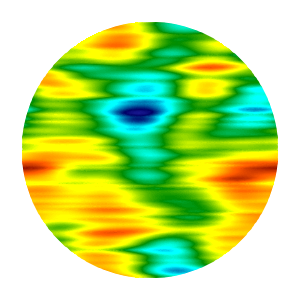
\includegraphics[width=\textwidth]{Chapter4/figures/2D/psic_brick.png}
    \caption{}
  \end{subfigure}
  \begin{subfigure}{0.15\textwidth}
    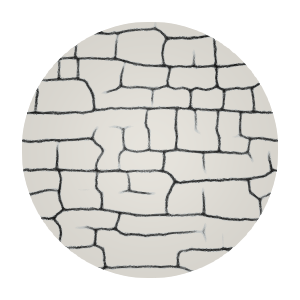
\includegraphics[width=\textwidth]{Chapter4/figures/2D/d_brick.png}
    \caption{}
  \end{subfigure}
  
  \begin{subfigure}{0.14\textwidth}
    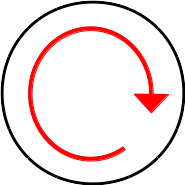
\includegraphics[width=\textwidth]{Chapter4/figures/2D/radial_schematic.png}
    \caption{}
  \end{subfigure}
  \hspace{0.02\textwidth}
  \begin{subfigure}{0.14\textwidth}
    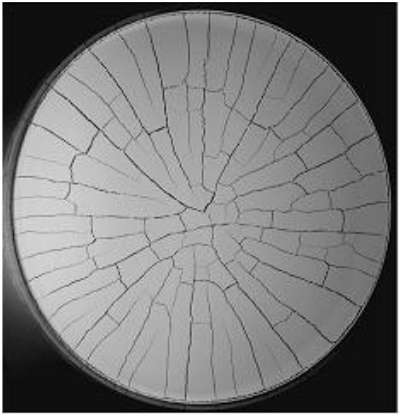
\includegraphics[width=\textwidth]{Chapter4/figures/2D/paste_radial.png}
    \caption{}
  \end{subfigure}
  \hspace{0.02\textwidth}
  \begin{subfigure}{0.15\textwidth}
    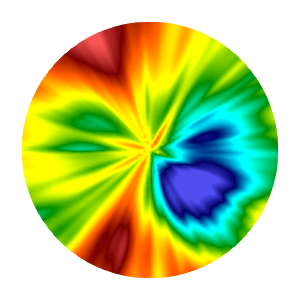
\includegraphics[width=\textwidth]{Chapter4/figures/2D/Gc_radial.png}
    \caption{}
  \end{subfigure}
  \begin{subfigure}{0.15\textwidth}
    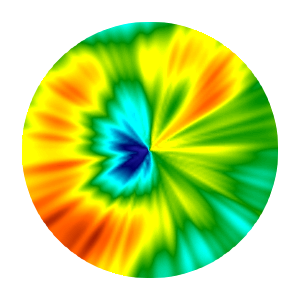
\includegraphics[width=\textwidth]{Chapter4/figures/2D/psic_radial.png}
    \caption{}
  \end{subfigure}
  \begin{subfigure}{0.15\textwidth}
    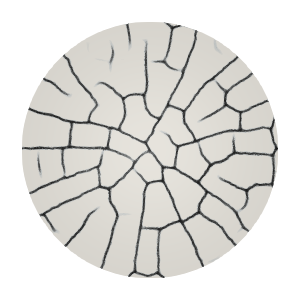
\includegraphics[width=\textwidth]{Chapter4/figures/2D/d_radial.png}
    \caption{}
  \end{subfigure}
  
  \begin{subfigure}{0.14\textwidth}
    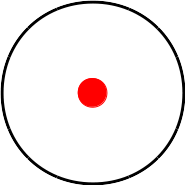
\includegraphics[width=\textwidth]{Chapter4/figures/2D/ring_schematic.png}
    \caption{}
  \end{subfigure}
  \hspace{0.02\textwidth}
  \begin{subfigure}{0.14\textwidth}
    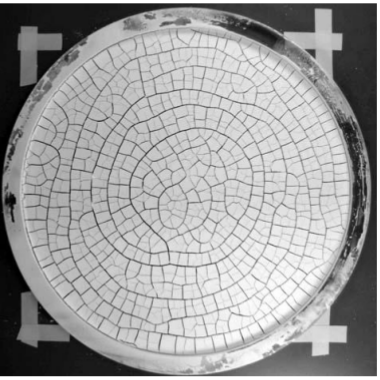
\includegraphics[width=\textwidth]{Chapter4/figures/2D/paste_ring.png}
    \caption{}
  \end{subfigure}
  \hspace{0.02\textwidth}
  \begin{subfigure}{0.15\textwidth}
    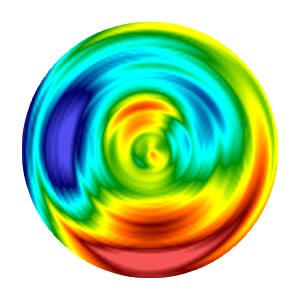
\includegraphics[width=\textwidth]{Chapter4/figures/2D/Gc_ring.png}
    \caption{}
  \end{subfigure}
  \begin{subfigure}{0.15\textwidth}
    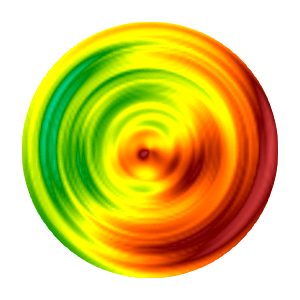
\includegraphics[width=\textwidth]{Chapter4/figures/2D/psic_ring.png}
    \caption{}
  \end{subfigure}
  \begin{subfigure}{0.15\textwidth}
    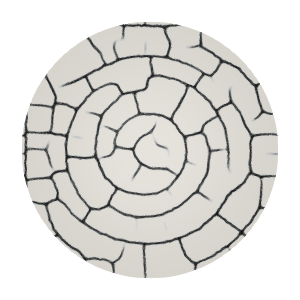
\includegraphics[width=\textwidth]{Chapter4/figures/2D/d_ring.png}
    \caption{}
  \end{subfigure}
  \caption[Three sets of experiments and calculations with different modes of agitation.]{Three sets of experiments and calculations for (a-e) unilateral agitation (f-j) rotational agitation (k-o) point agitation. (b, g, l) snapshots of crack patterns from experiments. postulated spatially correlated (c, h, m) fracture toughness and (d, i, n) critical fracture energy to reproduce experimental observations. (e, j, o) phase fields obtained using corresponding spatially varying material properties. }
  \label{fig: Chapter4/2D/japanese_experiments}
\end{figure}
